\chapter{Contexto y estado del arte}

En esta sección se intentarán poner en perspectiva, de una forma no exhaustiva, las distintas razones
históricas que dan lugar a la necesidad de crear un sistema de almacenamiento descentralizado y distribuido como IPFS.
Para ello, se hará un breve repaso histórico de la evolución de Internet y de los protocolos que lo han ido conformando.
Posteriormente, se explicará la tendencia centrlista del sistema actual, existente a un nivel íntrinseco y estructural,
además de otros problemas que se derivan de esta situación.
Finalmente, se expondrá la propuesta de solución que IPFS ofrece para solventar estos problemas, sobre la que se profundizará en el apartado \ref{sect:ipfs} dedicada a IPFS.

\section{Breve historia de Internet}
\subsection{Predominancia de los protocolos TCP/IP}
La historia de Internet está marcada por la competencia entre distintos protocolos de comunicación que buscaban establecerse
como el estándar para intercambiar información entre diferentes redes y sistemas. Uno de los episodios más relevantes de esta
competencia fue la llamada \textit{"Guerra de los protocolos"} \cite{ProtocolWars2023}, en la que el conjunto de protocolos TCP/IP, creado entre los
años 1973 y 1974 por Vint Cerf y Robert Kah, se enfrentó a otras propuestas como OSI, X.25 o SNA\footnote{En la figura \ref{tab:comparacion-protocolos-90} de la página \pageref{tab:comparacion-protocolos-90} se muestra un resumen de las principales características de cada uno de estos protocolos.
}.

TCP/IP logró imponerse en la competencia debido a las siguientes características principalmente:
\begin{itemize}
      \item \textbf{ Interoperabilidad }: La capacidad de TCP/IP para conectarse fácilmente con diferentes tipos de ordenadores y sistemas operativos le otorgaba una ventaja sobre otros protocolos que eran más específicos o limitados en su compatibilidad. Esta característica permitía que diversas tecnologías y plataformas pudieran comunicarse entre sí sin problemas, lo cual era esencial para crear una red global como Internet.

      \item \textbf{ Flexibilidad }: TCP/IP podía adaptarse a distintos medios de transmisión, como cables de cobre, fibra óptica o incluso enlaces inalámbricos, lo que facilitaba su implementación en una amplia variedad de entornos y situaciones. Otros protocolos, en cambio, podrían haber requerido modificaciones o adaptaciones específicas para funcionar en diferentes tipos de medios de transmisión.

      \item \textbf{ Resistencia }frente a fallos: TCP/IP fue diseñado para ser robusto en caso de fallos en la red, permitiendo que los paquetes de datos pudieran ser retransmitidos y encontrar rutas alternativas en caso de problemas. Esta capacidad de recuperación era fundamental para garantizar la continuidad y fiabilidad de las comunicaciones en una red global con múltiples nodos y enlaces.

      \item \textbf{ Escalabilidad }: TCP/IP podía soportar el crecimiento de la red al permitir la incorporación de nuevos nodos y enlaces sin afectar negativamente su rendimiento. Su diseño jerárquico y descentralizado facilitaba la expansión de la red y evitaba los cuellos de botella que podrían haberse producido con otros protocolos menos escalables.

\end{itemize}

Estas ventajas hicieron que TCP/IP se convirtiera en la opción preferida frente a otros protocolos, al ser una solución más versátil,
resistente y escalable para la creciente demanda de interconexión entre sistemas y redes en todo el mundo.
Cabe destacar también que era una solución con arquitectura abierta, no propietaria y de uso gratuito, es decir, sin necesidad de pagar licencias por su uso \cite{edwardsFoundationInternetTCP2021}.

Como en toda guerra también hubo un trasfondo político. Este hecho suele ser ignorado al abordarse este tema desde un punto de vista puramente tecnológico.
Y es que en 1980, el Departamento de Defensa de Estados Unidos declaró TCP/IP como el estándar para todas las redes militares \cite{leinerBriefHistoryInternet1999}.
A esto se sumaron numerosas comunidades de investigación y universidades que adoptaron TCP/IP como su protocolo de comunicación, como por ejemplo, Stanford University, donde Vint Cerf colaboró con Robert Kahn en el diseño del protocolo \cite{leinerBriefHistoryInternet1999}; University of California, Los Angeles (UCLA), que participó en el desarrollo temprano y las pruebas de TCP/IP \cite{leinerBriefHistoryInternet1999}; y University College London (UCL), donde el profesor Peter Kirstein promovió el uso de TCP/IP en Europa y su equipo contribuyó al desarrollo y pruebas del protocolo \cite{moriPeterKirsteinObituary2020}.

\begin{figure}[H]
      \centering
      \includegraphics[width=0.8\textwidth]{images/TimelineOfTheInternetProtocols.png}
      \caption[Evolución de los protocolos de Internet]{Evolución de los protocolos de Internet. Fuente \cite{leinerBriefHistoryInternet1999}}
\end{figure}

Esta completa adopción del protocolo se dió por finalizada cuando ARPANET la precursora de la actual Internet y financiada por la Agencia de Proyec
tos de Investigación Avanzados de Defensa (DARPA), llevó a cabo la transición exitosa de su antiguo protocolo, el Network Control Program (NCP),
a TCP/IP el 1 de enero de 1983
\cite{leinerBriefHistoryInternet1999}.

En resumen, la rápida adopción de la comunidad científica y academéica, sumada al respaldo gubernamental consolidaron TCP/IP como el estándar dominante en la industria de las redes de comunicación.

\subsection{La World Wide Web y HTTP}
El modelo TCP/IP asentó una forma de comunicación estándar entre computadores y redes, aunque
este estaba limitado principalmente al mundo académico y científico. No fue hasta la creación de la World Wide Web (WWW)
cuando el Internet concebido como es en la actualidad se convirtió en un fenómeno global y accesible para todo el mundo.

Antes de la WWW, el acceso a la información en Internet se realizaba a través de los protocolos a nivel de aplicación mostrados en la figura \ref{fig:evolucion-protocolos}

\begin{table}[h]
      \small
      \centering
      \begin{tabular}{>{\raggedright}m{3cm}m{10cm}}
            \toprule
            \textbf{Protocolo}                                   & \textbf{Descripción}                                                                                                                                                \\
            \midrule
            FTP (Protocolo de Transferencia de Archivos)         & Utilizado para transferir archivos entre cliente y servidor a través de una red.                                                                                    \\
            \addlinespace
            Telnet                                               & Basado en texto utilizado para el acceso remoto a computadoras y servidores, permitiendo a los usuarios controlarlos a través de una interfaz de línea de comandos. \\
            \addlinespace
            Gopher                                               & Diseñado para buscar y recuperar documentos de manera jerárquica, utilizando una interfaz basada en menús.                                                          \\
            \addlinespace
            SMTP (Protocolo Simple de Transferencia de Correo)   & Utilizado para enviar mensajes de correo electrónico entre servidores y, finalmente, al cliente de correo del destinatario.                                         \\
            \addlinespace
            NNTP (Protocolo de Transferencia de Noticias en Red) & Utilizado para la distribución, consulta y recuperación de artículos de noticias en la red Usenet.                                                                  \\
            \addlinespace
            POP3 (Protocolo de Oficina de Correos 3)             & Utilizado para recuperar mensajes de correo electrónico desde un servidor de correo remoto hasta un cliente de correo local.                                        \\
            \addlinespace
            IMAP (Protocolo de Acceso a Mensajes de Internet)    & Permite a los usuarios acceder y administrar sus mensajes de correo electrónico en un servidor de correo, sin descargarlos a un cliente de correo local.            \\
            \bottomrule
      \end{tabular}
      \caption{Protocolos de capa de aplicación antes de HTTP}
      \label{fig:evolucion-protocolos}
\end{table}

Estos servicios se encuentran dentro del nivel de aplicación  dentro del \textit{stack} TCP/IP, como se muestra en la figura \ref{fig:tcpip}.
Algunos de ellos se siguen usando hoy en día, o tienen su caso de uso (IMAP, POP3, FTP), pero en lo referente a archivos,
ofrecían métodos básicos de navegación y compartición, carecían de la capacidad de interconectar documentos de manera intuitiva y visual.
\footnote{Cabe destacar que en esta época, los documentos eran principalmente texto plano, sin formato, y no existía la posibilidad de incluir imágenes o vídeos.}

\usetikzlibrary{shapes,arrows,positioning, babel}
\begin{figure}[h!]
      \centering
      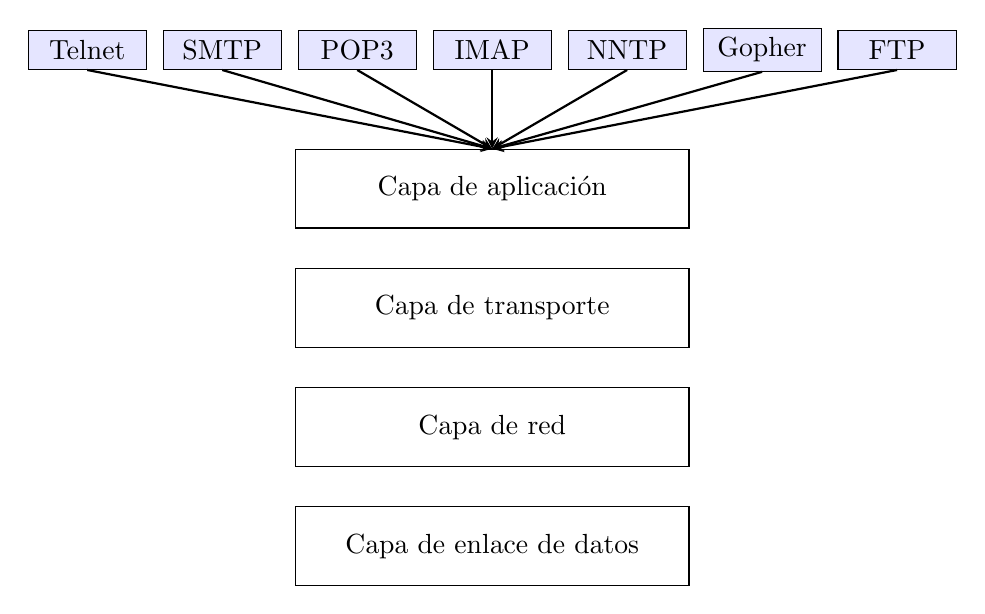
\begin{tikzpicture}
            % Estilos
            \tikzstyle{layer}=[draw, rectangle, minimum height=1cm, minimum width=5cm, text centered]
            \tikzstyle{app_protocol}=[draw, rectangle, minimum height=0.5cm, minimum width=1.5cm, text centered, fill=blue!10]
            \tikzstyle{arrow}=[->,>=stealth, thick]

            % Nodos
            \node[layer] (application) {Capa de aplicación};
            \node[layer, below=0.5cm of application] (transport) {Capa de transporte};
            \node[layer, below=0.5cm of transport] (network) {Capa de red};
            \node[layer, below=0.5cm of network] (link) {Capa de enlace de datos};

            \node[app_protocol, above=1cm of application.north] (imap) {IMAP};
            \node[app_protocol, left=0.2cm of imap] (pop3) {POP3};
            \node[app_protocol, right=0.2cm of imap] (nntp) {NNTP};
            \node[app_protocol, left=0.2cm of pop3] (smtp) {SMTP};
            \node[app_protocol, right=0.2cm of nntp] (gopher) {Gopher};
            \node[app_protocol, left=0.2cm of smtp] (telnet) {Telnet};
            \node[app_protocol, right=0.2cm of gopher] (ftp) {FTP};

            % Flechas
            \draw[arrow] (imap.south) -- (application.north);
            \draw[arrow] (pop3.south) -- (application.north);
            \draw[arrow] (nntp.south) -- (application.north);
            \draw[arrow] (smtp.south) -- (application.north);
            \draw[arrow] (gopher.south) -- (application.north);
            \draw[arrow] (telnet.south) -- (application.north);
            \draw[arrow] (ftp.south) -- (application.north);
      \end{tikzpicture}
      \caption{Capas del protocolo TCP/IP con algunos protocolos de la capa de aplicación}
      \label{fig:tcpip}
\end{figure}


En 1989, el científico británico Tim Berners-Lee propuso la creación de la WWW, un sistema de información global e hipertextual
que permitiría a los usuarios navegar y acceder a documentos interconectados mediante enlaces.



\section{IPFS como alternativa a HTTP}


\label{sect:ipfs}
\subsection{Introducción}
% Briefly introduce the concept of IPFS and its significance in the modern era of the internet.
% Provide a background on why IPFS was created and its aims.
\subsection{Fundamentos}
% Describe the key concepts and terminologies involved in IPFS, such as Content-addressed, Peer-to-peer (P2P) network, and Merkle DAG.
% Explain how these concepts work together to make IPFS a decentralized and distributed file system.
\subsection{Arquitectura}
% Describe the core components of IPFS architecture, such as IPFS node, IPFS client, IPFS gateway, and IPFS cluster.
% Explain the role of each component in the IPFS network.
\subsection{Modelo de datos}
% Explain the IPFS data model, which involves content addressing and hash-based naming.
% Discuss the benefits of the IPFS data model, such as data integrity, data verifiability, and content-based addressing.
\subsection{Distribución de contenido}
% Describe how IPFS handles content distribution and how it differs from the traditional client-server model.
% Explain how IPFS content distribution works in a P2P network.

\section{Ecosistema en torno a IPFS}

\subsection{Introducción}
% Introduce the concept of the IPFS ecosystem and why it is important.
% Briefly discuss the role of the ecosystem in the development and adoption of IPFS.
\subsection{Proyectos basados en IPFS} % Hablar de las DAPPS
% Provide an overview of the various IPFS projects that exist.
% Categorize the projects into different areas of application, such as storage, web hosting, content distribution, and decentralized applications (dApps).
% Provide examples of notable projects in each category and briefly describe their goals and features.
\subsection{Herramientas y librerías de IPFS}
% Discuss the various tools and libraries that are available to developers working with IPFS.
% Categorize the tools and libraries into different areas, such as API clients, command-line interfaces, development frameworks, and libraries for integrating IPFS into other applications.
% Provide examples of notable tools and libraries in each category and briefly describe their features and capabilities.
\subsection{Comunidades en torno a IPFS}
% Discuss the various communities that exist around IPFS.
% Categorize the communities into different areas, such as developer communities, user communities, and governance communities.
% Provide examples of notable communities in each category and briefly describe their goals and activities.
\subsection{Integraciones de IPFS}
% Discuss the various ways in which IPFS is being integrated with other technologies and platforms.
% Provide examples of notable integrations, such as with Ethereum, Filecoin, and the InterPlanetary Naming System (IPNS).
% Discuss the potential benefits of these integrations and their implications for the broader ecosystem.
